\documentclass{article}
\usepackage[utf8]{inputenc}
\usepackage{graphicx}
\usepackage{amsmath}
\usepackage{titling}
\usepackage{pdflscape}
\usepackage[export]{adjustbox}
\usepackage{float}
\usepackage{booktabs} % To thicken table lines
\usepackage{adjustbox}
\usepackage{caption}

\setlength{\droptitle}{-10em}
\pagestyle{empty}

\title{Lab. 4 - Clustering di dati medici}
\author{Ballarin Simone, Gobbo Alessio, Rossi Daniel}
\date{June 2019}

\begin{document}

\maketitle

\section*{Domanda 1}
Viene riportato il grafico ottenuto dall'esecuzione dell'algoritmo Gerarchico.\\
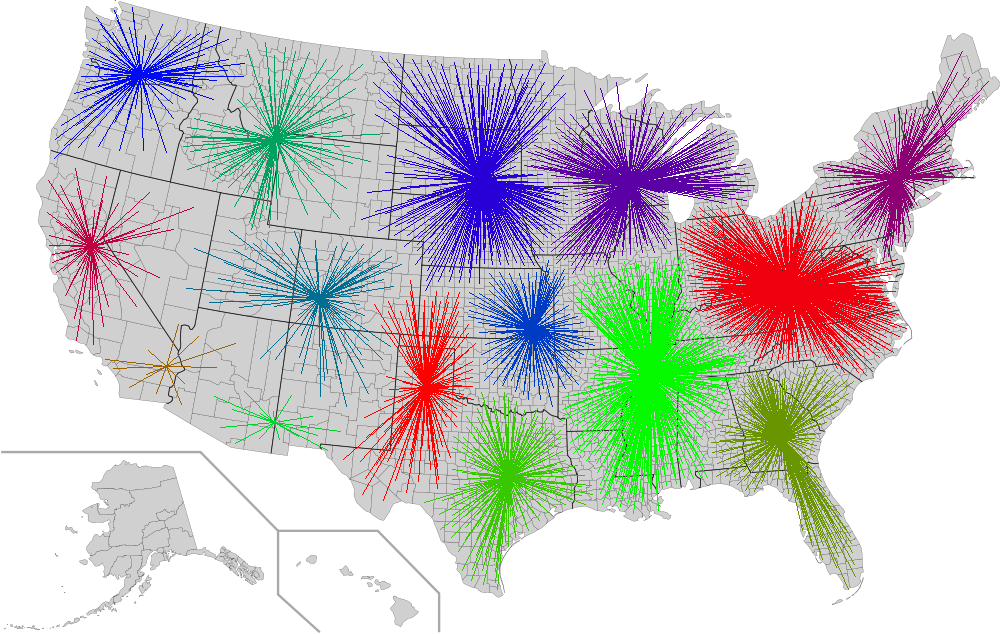
\includegraphics[width=1.0\linewidth, valign=t]{figures/Domanda1}

\section*{Domanda 2}
Viene riportato il grafico ottenuto dell'esecuzione dell'algoritmo Kmeans.\\
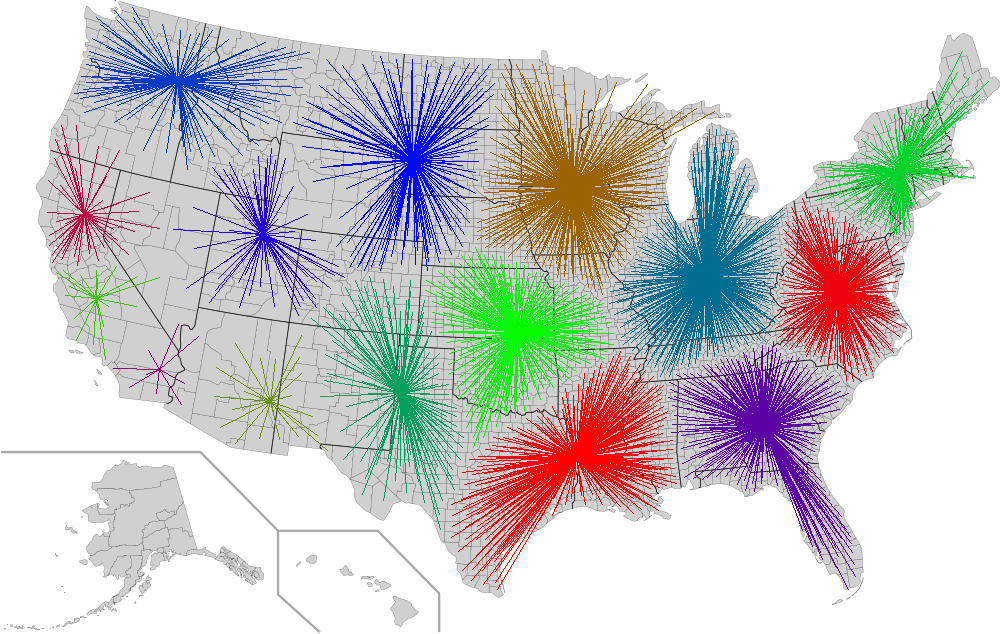
\includegraphics[width=1.0\linewidth, valign=t]{figures/Domanda2}

\section*{Domanda 3}
Dati $q$ il numero di iterazioni di \textit{kmeans}, $k$ il numero di clustering e $n$ la cardinalità dell'insieme dei punti, possiamo quantificare le seguenti complessità dei due algoritmi di clustering:
\begin{itemize}
\item La complessità del clustering gerarchico è $O(n\,h(n))$, dove $h(n)$ è la complessità della ricerca dei punti più vicini.
Questa ricerca è stata effettuata con la funzione \textit{FastestClosestPair}, la quale ha complessità $O(n\,log(n))$;
Quindi complessivamente il clustering gerarchico ha complessità $O(n^2\,log(n))$.
\item La complessità di \textit{kmeans} invece è di $O(q\,n\,k)$. 
\end{itemize}

\noindent Ipotizzando quindi $q$ e $k$ fattori molto piccoli, quindi trascurabili come segue $q \approx 1$ e $k \approx 1$, giungiamo alla conclusione che 
la complessità del clustering gerarchico rimanga inalterata, mentre \textit{kmeans} giunga a $O(n)$.\\
Da quando appena esposto risulta evidente come \textit{kmeans} sia in termini asintotici, e considerando $q$ e $k$ insignificanti, significativamente piu' efficienti.

\section*{Domanda 4}
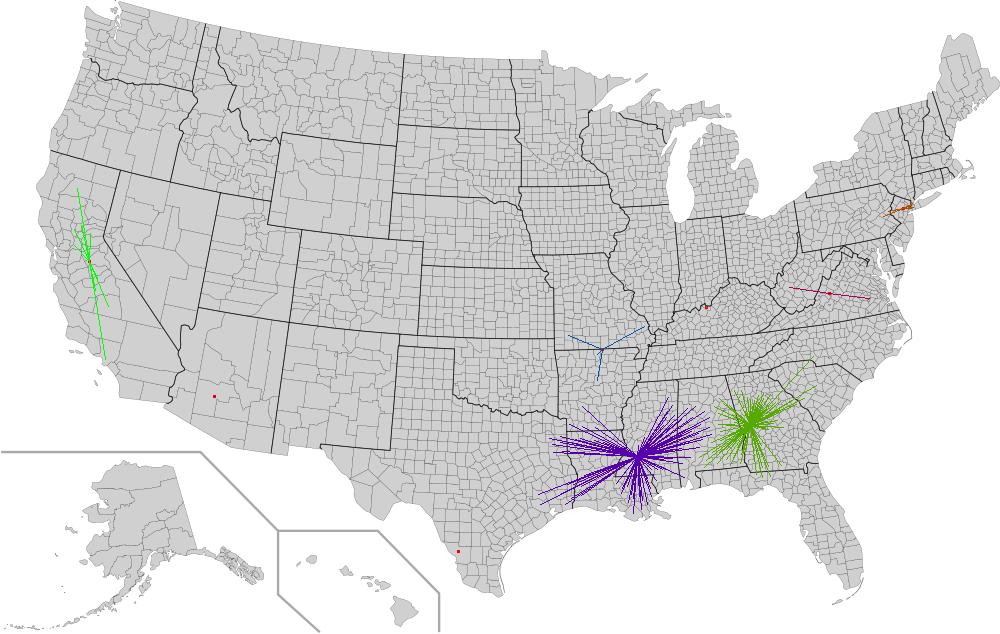
\includegraphics[width=1.0\linewidth, valign=t]{figures/Domanda4}

\section*{Domanda 5}
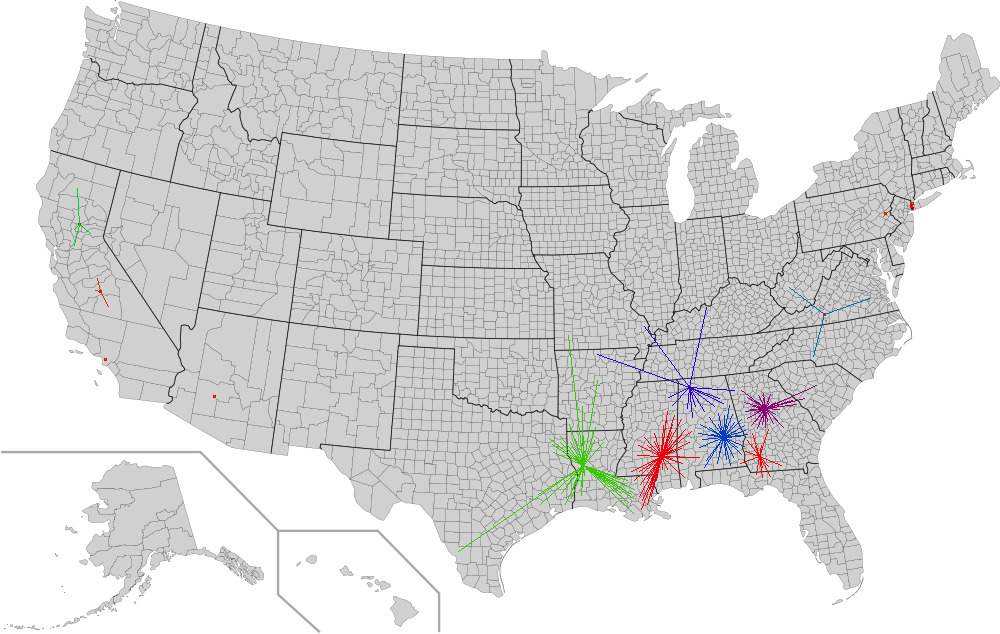
\includegraphics[width=1.0\linewidth, valign=t]{figures/Domanda5}

\section*{Domanda 9}
Di seguito vengono riportati tre grafici, ognuno facente riferimento ad un dataset di dimensioni differenti (in sequenza 212, 562 e 1041 contee). 
Ogni grafico esprime sull'asse delle ordinate il valore della metrica dispersione al variare del numero di cluster in output. \newline
\subsection*{212 contee, clustering gerarchico e k-means}
\begin{figure}[H]
	\hspace*{-1cm}\begin{minipage}{0.55\linewidth}
		\centering
			\begin{tabular}{lrr}
	\toprule
	{} & hierarchical & kmeans       \\
	k  &              &              \\
	\midrule
	6  & 3.551330e+11 & 1.942049e+11 \\
	7  & 2.119842e+11 & 1.216588e+11 \\
	8  & 2.079946e+11 & 1.208180e+11 \\
	9  & 1.967522e+11 & 9.538277e+10 \\
	10 & 1.458858e+11 & 7.612516e+10 \\
	11 & 7.333959e+10 & 6.940441e+10 \\
	12 & 7.298695e+10 & 5.684592e+10 \\
	13 & 6.292566e+10 & 5.105708e+10 \\
	14 & 3.749038e+10 & 4.506050e+10 \\
	15 & 3.075468e+10 & 4.144032e+10 \\
	16 & 3.052271e+10 & 3.658922e+10 \\
	17 & 1.965371e+10 & 3.645427e+10 \\
	18 & 1.899275e+10 & 1.849405e+10 \\
	19 & 1.890876e+10 & 1.754538e+10 \\
	20 & 1.449351e+10 & 1.612765e+10 \\
	\bottomrule
\end{tabular}

	\end{minipage}
	\begin{minipage}{0.7\linewidth}
		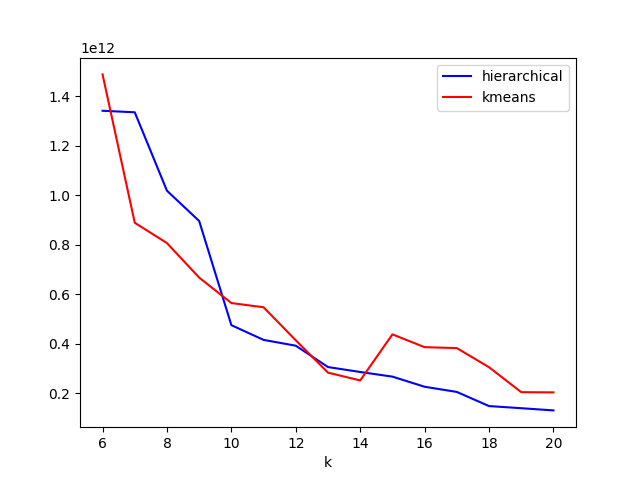
\includegraphics[width=1.0\linewidth, valign=t]{figures/output562}
		\caption*{Grafico dispersione del dataset con 212 contee.}
	\end{minipage}
\end{figure}
\subsection*{562 contee, clustering gerarchico e k-means}

\begin{figure}[H]
	\hspace*{-1cm}\begin{minipage}{0.55\linewidth}
		\centering
        \begin{tabular}{lrr}
\toprule
{} &  hierarchical &        kmeans \\
k  &               &               \\
\midrule
6  &  1.341235e+12 &  1.488108e+12 \\
7  &  1.335053e+12 &  8.888297e+11 \\
8  &  1.018233e+12 &  8.067753e+11 \\
9  &  8.959328e+11 &  6.674107e+11 \\
10 &  4.751940e+11 &  5.644963e+11 \\
11 &  4.157366e+11 &  5.475082e+11 \\
12 &  3.922197e+11 &  4.140267e+11 \\
13 &  3.060045e+11 &  2.835009e+11 \\
14 &  2.860567e+11 &  2.519570e+11 \\
15 &  2.673648e+11 &  4.380518e+11 \\
16 &  2.264599e+11 &  3.862867e+11 \\
17 &  2.055237e+11 &  3.826377e+11 \\
18 &  1.484142e+11 &  3.053247e+11 \\
19 &  1.397912e+11 &  2.046021e+11 \\
20 &  1.309398e+11 &  2.037350e+11 \\
\bottomrule
\end{tabular}
 
    \end{minipage}
        \begin{minipage}{0.7\linewidth}
            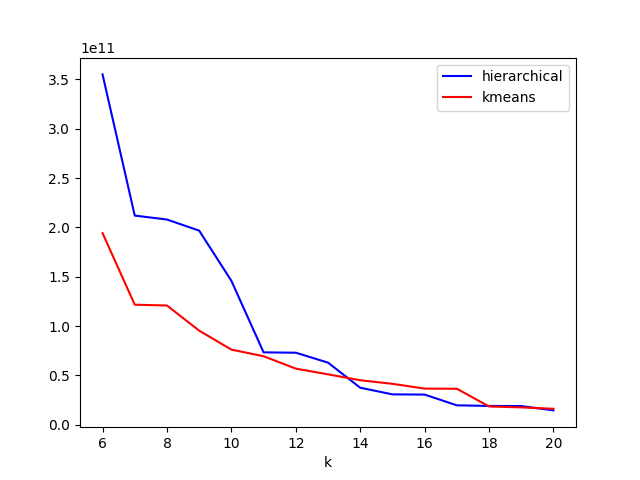
\includegraphics[width=1.0\linewidth, valign=t]{figures/output212}
			\caption*{Grafico dispersione del dataset con 562 contee.}
		\end{minipage}
\end{figure}
\subsection*{1041 contee, clustering gerarchico e k-means }
\begin{figure}[H]
	\hspace*{-1cm}\begin{minipage}{0.55\linewidth}
		\centering
			\begin{tabular}{lcc}
	\toprule
	k  & Gerarchico   & Kmeans       \\
	\midrule
	6  & 2.497247e+12 & 2.524928e+12 \\
	7  & 2.222620e+12 & 1.568259e+12 \\
	8  & 1.375668e+12 & 1.180744e+12 \\
	9  & 1.140418e+12 & 1.089885e+12 \\
	10 & 8.687074e+11 & 8.469028e+11 \\
	11 & 8.461629e+11 & 7.754888e+11 \\
	12 & 8.407428e+11 & 7.742760e+11 \\
	13 & 8.309796e+11 & 7.727588e+11 \\
	14 & 6.195937e+11 & 7.119578e+11 \\
	15 & 5.753650e+11 & 6.438951e+11 \\
	16 & 5.010563e+11 & 6.243352e+11 \\
	17 & 4.670626e+11 & 4.585690e+11 \\
	18 & 4.216256e+11 & 4.254108e+11 \\
	19 & 3.703708e+11 & 4.204501e+11 \\
	20 & 3.666637e+11 & 3.834206e+11 \\
	\bottomrule
\end{tabular}

	\end{minipage}
	\begin{minipage}{0.7\linewidth}
		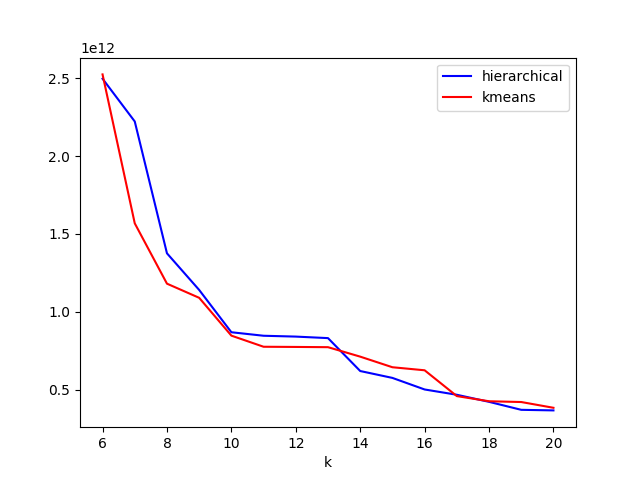
\includegraphics[width=1.0\linewidth, valign=t]{figures/output1041}
		\caption*{Grafico dispersione del dataset con 1041 contee.}

	\end{minipage}
\end{figure}


\end{document}